\section{Multiple Correspondence Analysis}
\label{sec:multivariate}

In this section I perform multiple correspondence analysis for same variables than were discussed in section \ref{sec:bivariate}. In figure \ref{fig:mca} a visualization of the result of the multiple correspondence analysis between game result, game variant, time of day and color of pieces is shown. I propose following interpretation for the two axes that explain data best. Dimension 1 describes how likely game is to result in a draw. This makes clear distinction between crazyhouse chess and other studied variants because crazyhouse game is very unlike to end in a draw. Dimension 2 can be interpreted as winning-losing axel. Winning is most clearly aligned with having white pieces and somewhat aligned with playing standard chess with long time control. Losing is related to having black pieces and it is somewhat related to playing standard chess with short time control. I don't provide any interpretation for direction related time of day. In this plot connection between losing and crazyhouse chess seen in figure \ref{fig:variant vs result} is not present anymore. This acts as a remainder to be careful when making conclusions from correspondence analysis plots as MCA is non robust method and it is affected a lot by our earlier decision like on how to aggregate data to different categories and how we select threshold for rating difference after which we consider opponent stronger.

\begin{figure}[ht!]
    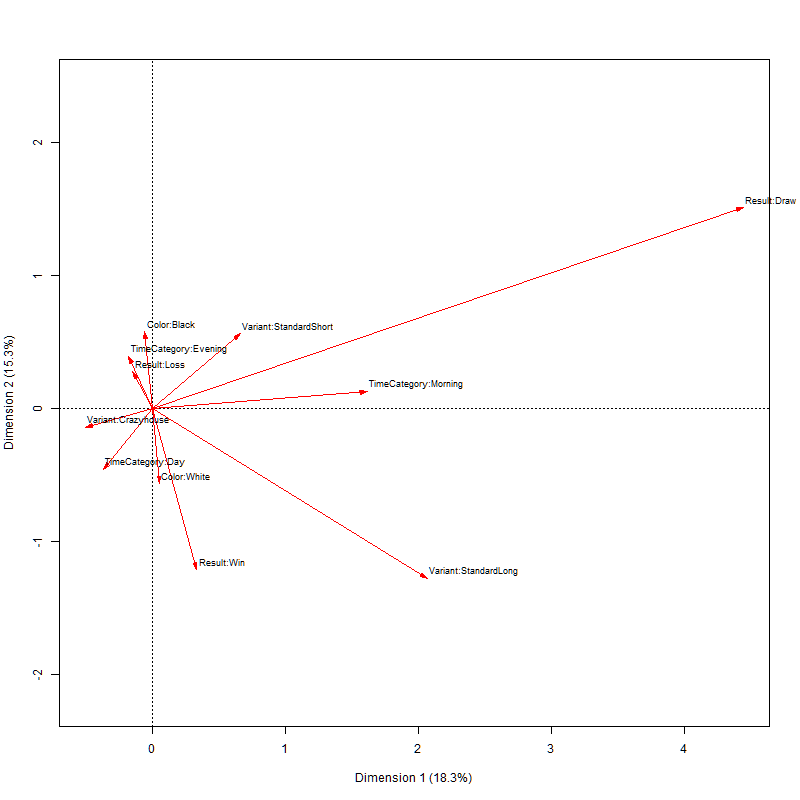
\includegraphics[width=\textwidth]{../img/mca.png}
    \caption{Visualization of the result of the multiple correspondence analysis between game result, game variant, time of day and color of pieces.}
    \label{fig:mca}
\end{figure}